\documentclass[a4paper]{iutvexam}
% compile-latex options:--jobname controle20141121
% compile-latex options:--jobname correction20141121
\usepackage{graphicx}
\usepackage{listings}
\usepackage{textcomp,tikz}

\title{Contrôle 2}
\date{21/11/2014}
\begin{document}
\conditions{ Vous disposez de 2 heures pour faire ce contrôle. Aucun
  document autorisé. Toute tentative de communication avec un voisin ou
  l'extérieur peut être sanctionnée. Toutes les réponses doivent être
  faites sur l'énoncé. La taille de la réponse attendue dépend de la
  taille allouée pour répondre. }
\begin{questions}
  \titledquestion{Système}
  \begin{parts}
    \part[3] Rappelez les principales différences entre code compilé et code interprété (avantages / inconvénients)
    \begin{solutionordottedlines}[1.5in]%
      C'est dans le cours. Les trois mots clés : portabilité, efficacité, cycle de développement
    \end{solutionordottedlines}
    \part[\half] Sous Linux, comment le système reconnaît-il le type de données dans un fichier: par son extension, par son nom, par son contenu, par des métadonnées, par son numéro d'inode ? Est-ce que cette réponse est vraie sous tous les systèmes ?
    \begin{solutionordottedlines}[.25in]%
      Par son contenu, et non. (Oui, c'est du premier contrôle)
    \end{solutionordottedlines}

    \part[\half] Quel est le chemin absolu du fichier que vous avez utilisé pour modifier votre chemin d'exécution (PATH) ?
    \begin{solutionordottedlines}[.25in]%
      \verb|~/.bashrc|
    \end{solutionordottedlines}

    \part[1] Quel est le nom des trois canaux de communication (flux) ouverts par défaut pour tout processus ?
    \begin{solutionordottedlines}[.25in]%
      STDIN, STDOUT, STDERR (accepter entrée standard, sortie standard, sortie erreur)
    \end{solutionordottedlines}
  \end{parts}

  \titledquestion{Textes}
  Un système d'encodage de texte utilise la convention suivante : «~tous les caractères peuvent être codés par \verb|>XXXX| où XXXX est le numéro \textbf{hexadécimal} du caractère en unicode (forcément sur 4 chiffres). Le caractère \verb|>| doit obligatoirement être échappé de cette façon.~»
  Trois numéros \emph{hexadécimaux} de caractères qui seront utiles dans l'exercice : € a pour numéro \texttt{20AC}, \texttt{é} a pour numéro \texttt{E9}, \texttt{A} a pour numéro \texttt{41}.
  \begin{parts}
    \part[\half] Que veut dire la chaîne «~\verb|Pay>00E9: 20>20AC|~»?
    \begin{solutionordottedlines}[.25in]%
      Payé: 20€
    \end{solutionordottedlines}
    \part[1] Sachant que le code \emph{décimal} du caractère \verb|%| est 62, donnez l'encodage de la chaîne suivante : «~\verb|1€>10c|~».
    \begin{solutionordottedlines}[.25in]%
      \verb|1>20AC>003E10c|
    \end{solutionordottedlines}
    \part[2] Complétez le schéma suivant:
    \begin{center}
      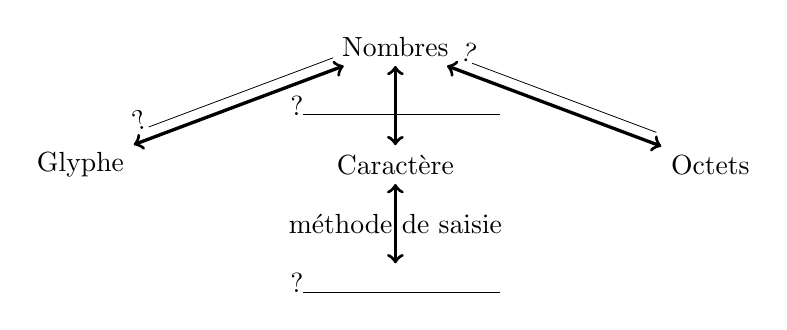
\begin{tikzpicture}
        \tikzstyle{every node}=[rounded corners]
        \tikzstyle{xlabel}=[]
        \tikzstyle{normally}=[very thick]
        \node (a) at (0,0) {Glyphe};
        \node (b) at (4,1.5) {Nombres}
        edge  [<->,normally] node[xlabel,above,sloped] {?\rule{25mm}{.1mm}} (a);
        \node (c) at (4,0) {Caractère}
        edge  [<->,normally] node[xlabel] {?\rule{25mm}{.1mm}} (b);
        \node (d) at (4,-1.5) {?\rule{25mm}{.1mm}}
        edge  [<->,normally] node[xlabel] {méthode de saisie} (c);
        \node (d) at (8,0) {Octets}
        edge  [<->,normally] node[xlabel,above,sloped] {?\rule{25mm}{.1mm}} (b);
      \end{tikzpicture}
    \end{center}
  \end{parts}
  \titledquestion{Formats}
  \begin{parts}
    \part[\half] Parmi les formats d'images bitmap sans perte, citez-en un avec compression possible, et un autre sans
    \begin{solutionordottedlines}[.25in]%
      PNG/PBM (0 si on n'a pas deux formats) (PBM peut être nommé « le format vu en exercice » ou équivalent)
    \end{solutionordottedlines}

    % \part[\half] Parmi les formats audio, citez-en un avec perte, et un autre sans perte
    % \begin{solutionordottedlines}[.25in]%
    %   MP3/FLAC (ou WAV)
    % \end{solutionordottedlines}

    % \part[\half] Parmi les formats audio sans perte, citez-en un avec compression possible, et un autre sans
    % \begin{solutionordottedlines}[.25in]%
    %   FLAC/WAV
    % \end{solutionordottedlines}

    \part[\half] Parmi les formats d'images compressés, citez-en un avec perte, et un autre sans perte
    \begin{solutionordottedlines}[.25in]%
      JPEG/PNG
    \end{solutionordottedlines}

    \part[1\half] Donnez un format le plus adapté pour ces trois images:\\
    \begin{center}
      \begin{tabular}{c|c|c}
        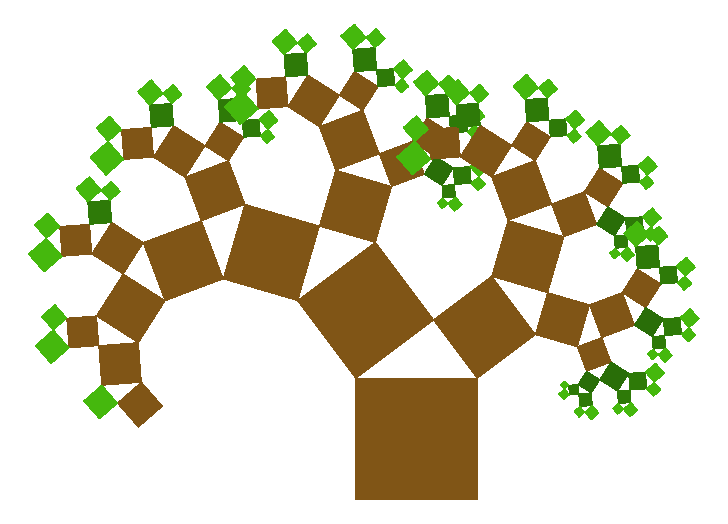
\includegraphics[width=.25\linewidth]{img/ctrl/PythagoreanTreeB6.pdf} &
        
\includegraphics[width=.25\linewidth]{img/ctrl/lord-attack-mace.png} &
        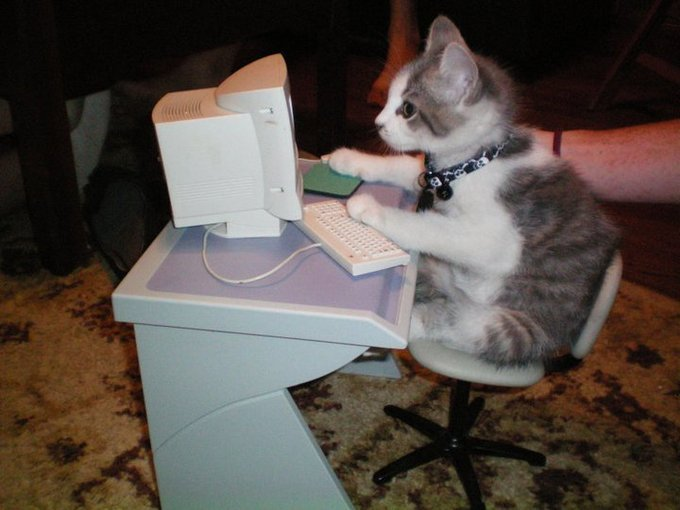
\includegraphics[width=.25\linewidth]{img/ctrl/kitten.jpg}
      \end{tabular}
    \end{center}
    \begin{solutionordottedlines}[.25in]%
      Vectoriel (ici c'est un PDF), PNG, JPG
    \end{solutionordottedlines}

    \part[1\half] En quelques mots, quel est le principe d'un filtrage haute fréquence (donnez un exemple pour l'audio et un exemple pour les images) ?
    \begin{solutionordottedlines}[.75in]%
      Le principe est de ne pas représenter des variations de signal qui
      seraient de toutes façons difficilement perceptibles. Pour le son,
      on peut par exemple ne pas représenter les fréquences
      inaudibles. Pour l'image, on peut par exemple ne pas représenter
      de petites différences de couleur dans des pixels contigus.
    \end{solutionordottedlines}
    \part[1\half] Que signifient les initiales RGB, CMY et HSL (en anglais, on trouve aussi HSV) ou bien RVB, CMJ et TSV (en français) ?

    \begin{solutionordottedlines}[.5in]%
      RedGreenBlue/CyanMagentaYellow/HueSaturationLightness ou bien RougeVertBleu/CyanMagentaJaune/TeinteSaturationValeur
    \end{solutionordottedlines}


    \part[1] Si une couleur a besoin de beaucoup d'encre Cyan pour
    être reproduite sur une feuille de papier, que sait-on sur une de
    ses composantes RVB en HTML ?
    \begin{solutionordottedlines}[.25in]%
      Bcp de Cyan -> Peu de Red. On ne sait pas grand chose sur le reste.
    \end{solutionordottedlines}

    \part[1] Petits, quand vous mélangiez des couleurs primaires à la gouache pour obtenir dez nouvelles couleurs, utilisiez-vous un système additif ou soustractif ? Expliquez en quelques mots.
    \begin{solutionordottedlines}[.75in]%
      Soustractif : chaque couleur soustrayait de la lumière naturelle certaines longueurs d'ondes
    \end{solutionordottedlines}

    \part[\half] En mélangeant des quantités maximales RVB, quelle couleur obtient-on ? En mélangeant des quantités maximales CMY, quelle couleur obtient-on ?
    \begin{solutionordottedlines}[.25in]%
      blanc/noir
    \end{solutionordottedlines}
  \end{parts}
  \titledquestion{Représentation mémoire}
  \begin{parts}
    \part[1\half] Quelle est la plus petite quantité d'information stockable dans un système informatique ? Quelle est la quantité d'information la plus petite que l'on peut désigner naturellement dans un système ? Comment s'appelle la taille \emph{habituellement} manipulée par le processeur ?
    \begin{solutionordottedlines}[.5in]%
      bit / octet / mot-machine (32 bits ou 64 bits selon les processeurs) (accepter taille d'un registre ou taille d'un \texttt{int})
    \end{solutionordottedlines}
    \newpage
    \part[3] Est-ce qu'il existe des petits-boutiens (\emph{little endian}) ou grands-boutiens (\emph{big endian}) sur un processeur 32 bits ? 16 bits ? 8 bits ? Expliquez.
    \begin{solutionordottedlines}[.75in]%
      On ne peut pas avoir deux ordres de rangement des octets faisant partie d'une même donnée si on n'a pas au moins deux octets à ranger. Au moins 1,5 pour l'explication.
    \end{solutionordottedlines}
    \part[3] Soit la donnée suivante:
    \begin{lstlisting}[language=C]
      typedef struct blob {
        char content;
        char number;
        blob* other;
        unsigned char tag;
        int id;
      } Blob;
    \end{lstlisting}
    Représentez la disposition en mémoire (trous compris) de cette
    structure \emph{Blob} si on suppose que les pointeurs et les entiers
    occupent tous deux 4 octets.
    \begin{solutionordottedlines}[1in]%
      char, char, trou, trou, 4 octets d'adresse, char, trou, trou, trou, 4 octets d'int.
    \end{solutionordottedlines}
    \part[\half] À la question précédente, quelle est la taille totale utilisée de la structure ?
    \begin{solutionordottedlines}[.25in]%
      
    \end{solutionordottedlines}

    \part[\half] Quel type de processeur a des valeurs différentes de 4 octets pour les pointeurs et les \texttt{int} ? Est-ce que la taille de la structure peut dépendre du système d'exploitation ?
    \begin{solutionordottedlines}[.25in]%
      Les processeurs 64 bits, par exemple.
    \end{solutionordottedlines}
  \end{parts}
  \titledquestion{Script} On dispose dans un répertoire de fichiers de
  renseignement sur des étudiants. Les fichiers sont nommés du numéro de
  chaque étudiant, et contiennent des renseignements (un par ligne,
  toujours dans le même ordre).
  \begin{parts}
    \part[1\half] Faire un script qui affiche \verb|Nombre de lignes par fichier: 37| en calculant le 37 en regardant dans un des fichiers spécifié sur la ligne de commande. On rappelle qu'il existe une option \verb|-n| à la commande d'affichage pour ne pas aller à la ligne...
    \begin{solutionordottedlines}[1.5in]%
      
    \end{solutionordottedlines}
    \part[1] Donnez un extrait de script qui met dans une variable TEST le nom du premier fichier dans l'ordre donné par \verb|*|
    \begin{solutionordottedlines}[.75in]%
      
    \end{solutionordottedlines}
    \part[4] On rappelle que la syntaxe \verb|$(...)| %$
    permet de récupérer le contenu textuel d'une autre commande (et de
    le mettre par exemple dans une variable) (dans certains groupes, il
    a été vu le \verb|`...`|).  Faites un script qui vérifie que tous
    les fichiers du répertoire ont bien le même nombre de lignes : si
    c'est le cas on n'affiche rien, sinon on affiche le nom du (ou des)
    fichiers qui sont différents de celui pris comme référence. Vous
    pouvez supposer que le nom du fichier de référence est dans une
    variable TEST (comme expliqué à la question précédente).
    \begin{solutionordottedlines}[3in]%
      
    \end{solutionordottedlines}
    % tester les tuyaux
    \part[2] Faire un script à qui on donne le numéro de l'étudiant comme argument, et qui affiche son nom et son prénom, information qui est stockée à la troisième ligne du fichier (pas de vérification d'erreur demandée).
    \begin{solutionordottedlines}[1.5in]%
      
    \end{solutionordottedlines}
    % tester les tests
    \part[2] On veut modifier le script précédent pour qu'il vérifie que l'étudiant dont on a donné le numéro existe bien. Que faut-il rajouter au début ?
    \begin{solutionordottedlines}[1in]%
      
    \end{solutionordottedlines}
    % tester la généricité
    \part[2\half] Comment feriez-vous si on vous disait maintenant qu'on a plusieurs promotions, et que les fiches d'étudiants sont rangées dans des répertoires, un par promotion, pour que les scripts continuent à fonctionner ? (il n'est pas nécessaire d'écrire du code ici)
    \begin{solutionordottedlines}[1.5in]%
      
    \end{solutionordottedlines}
  \end{parts}
\end{questions}
\end{document}
